\chapterimage{img/SuperKK.jpg} % Chapter heading image
\chapterspaceabove{6.75cm} % Whitespace from the top of the page to the chapter title on chapter pages
\chapterspacebelow{7.25cm} % Amount of vertical whitespace from the top margin to the start of the text on chapter pages

%------------------------------------------------

\chapter{Raggi cosmici}\index{Raggi cosmici}

In questo capitolo si affronta il primo argomento trattato dal corso: i raggi cosmici. Lo scopo è quello di dare informazioni sui vari esperimenti condotti a terra sulla misurazione di proprietà importanti degli sciami originati da particelle provenienti dallo spazio, nonchè studiare alcuni tra i principali meccanismi di accelerazione di queste particelle. L'obiettivo principale è quello di comprendere e modellizzare l'andamento dello spettro in energia in Fig.(\ref{img:cosmicrays}).

\section{Rivelazione di raggi cosmici}

Come si misurano i raggi cosmici? Non esiste una risposta esaustiva, ovviamente dipende da dove vengono rivelati.
\begin{itemize}
    \item Misurazioni fuori dall'atmosfera:
    \begin{itemize}
        \item assenza di atmosfera,
        \item dimensioni limitate per problemi logistici e di costo.
    \end{itemize}
    \item Con palloni aerostatici:
    \begin{itemize}
        \item basso costo, atmosfera residua limitata,
        \item brevi periodi di vita ($\sim$ settimane).
    \end{itemize}
    \item Dal suolo terrestre:
    \begin{itemize}
        \item larghe aree coperte (ordine del km$^2$),
        \item schermo dell'atmosfera, si osservano i prodotti secondari.
    \end{itemize}
    \item Dal sottosuolo:
    \begin{itemize}
        \item grossi volumi, adatti per fisica dei neutrini,
        \item difficoltà tecniche per luogo e dimensioni.
    \end{itemize}
\end{itemize}
Quando si progetta un esperimento che vuole rivelare particelle provenienti dalle regioni dello spettro a maggior energia, facendo riferimento a Fig.(\ref{img:cosmicrays}), bisogna tener di conto del flusso di tali particelle: sarebbe ad esempio impensabile di condurre dallo spazio un esperimento per la misura di particelle con energie dell'ordine di $10^{18}\,\textup{eV}$, essendo che siamo in grado di mandare in orbita strumentazioni con dimensioni ridotte (si noti dalla figura che in questo caso stiamo cercando di misurare flussi dell'ordine di $1\,\textup{evt}/\textup{y}\cdot\textup{km}^2$). Dobbiamo dunque, in questo caso, accettare il fatto di fare la misura da terra e convivere con la presenza di particelle secondarie.

Quando un nucleo proveniente dallo spazio incontra l'atmosfera terrestre infatti dà luogo ad uno sciame. Come visto in precedenza ci sono alcuni processi importanti, due esempi da tenere bene a mente sono i seguenti:
\begin{gather*}
    \pi^{+} \rightarrow \mu^+ + \nu_\mu, \\
    \mu^+   \rightarrow e^+ + \bar{\nu}_\mu + \nu_e,
\end{gather*}
e ovviamente i rispettivi processi con il coniugato di carica. Dunque possiamo assumere che l'atmosfera in questo si comporta proprio come un calorimetro. Il massimo di uno sciame, come già accennato in precedenza, si ha ad una profondità proporzionale al logaritmo dell'energia della particella incidente. La maggior parte degli esperimenti condotti dal suolo terrestre si trova su altopiani, con lo scopo di rivelare il maggior numero di particelle provenienti da uno sciame e di ridurre le fluttuazioni statistiche dovute alla frazione elettromagnetica dello sciame.

\section{Esperimenti sui raggi cosmici}\index{Raggi cosmici!Esperimenti}

Gli esperimenti che si svolgono sul suolo, sono posti alla massima altezza possibile (ordine di $2-3\,\textup{km}$), alcuni siti di esempio sono in Argentina e Cile. Questi esperimenti mappano un terreno vasto con un certo numero di rivelatori, misurando informazioni di spazio (rivelatore colpito), tempo (intervallo di tempo in cui il segnale è presente in un singolo rivelatore) e ampiezza del segnale (proporzionale al numero di particelle che attraversano il singolo rivelatore) è possibile ricostruire l'evoluzione spaziale dello sciame, tipicamente con un errore di circa $1^\circ$.

L'esperimenti di Auger vuole osservare sciami provenienti da particelle con energie dell'ordine di $10^{18}\,\textup{eV}$. Per fare ciò usa un \emph{array} di 1600 rivelatori (contenitori di acqua pura, effetto Cherenkov) dispersi in un'area di $3000\,\textup{km}^2$. In Fig.(\ref{img:auger}) si riportano due foto dell'esperimento.
\begin{figure}[H]
    \centering
    \subfloat[\centering Sito dell'esperimento di Auger.]{{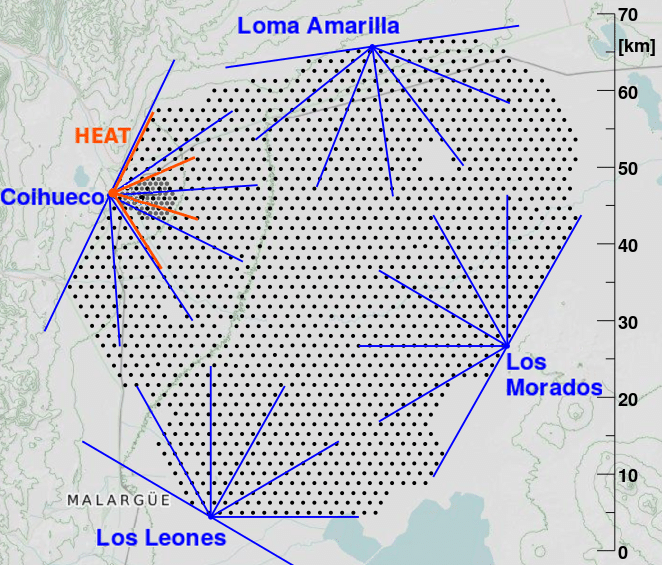
\includegraphics[width=0.4\textwidth]{img/auger_site.png} }}%
    \qquad
    \subfloat[\centering Foto di un detector di Auger.]{{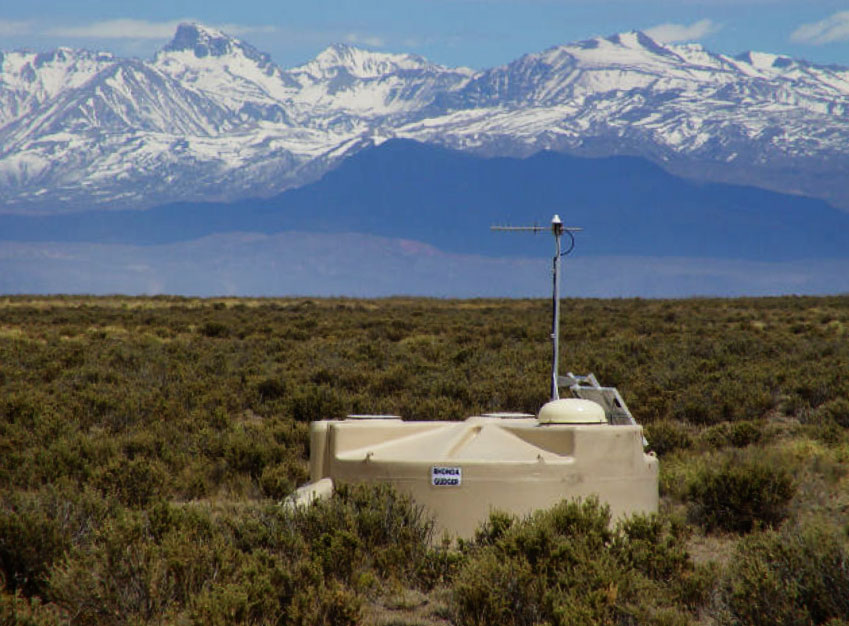
\includegraphics[width=0.45\textwidth]{img/auger_detector.jpg} }}%
    \caption{Immagini dell'esperimento \href{https://www.auger.org}{Auger}, situato in Argentina.}%
    \label{img:auger}
\end{figure}
Ciascun rivelatore contiene acuqa, con un PMT che rivela la luce emessa per effetto Cherenkov. Dalla misura dell'energia depositata nei rivelatori e dal tempo di arrivo del segnale, si riesce a risalire alla direzione di provenienza del raggio cosmico, alla sua energia e, con una certa approssimazione, anche al suo $Z$.

Un altro esempio di esperimento è KASKADE, in Germania. Un array di 252 rivelatori in un'area di $200\times 200\,\textup{m}^2$, ciascun rivelatore consiste in un calorimetro adronico composto di ferro e camere di ionizzazione. Data l'area minore di estenzione dell'esperimento, non è possibile rivelare sciami provenienti da particelle con energia dell'ordine di $10^{20}\,\textup{eV}$.

\begin{figure}[H]
    \centering
    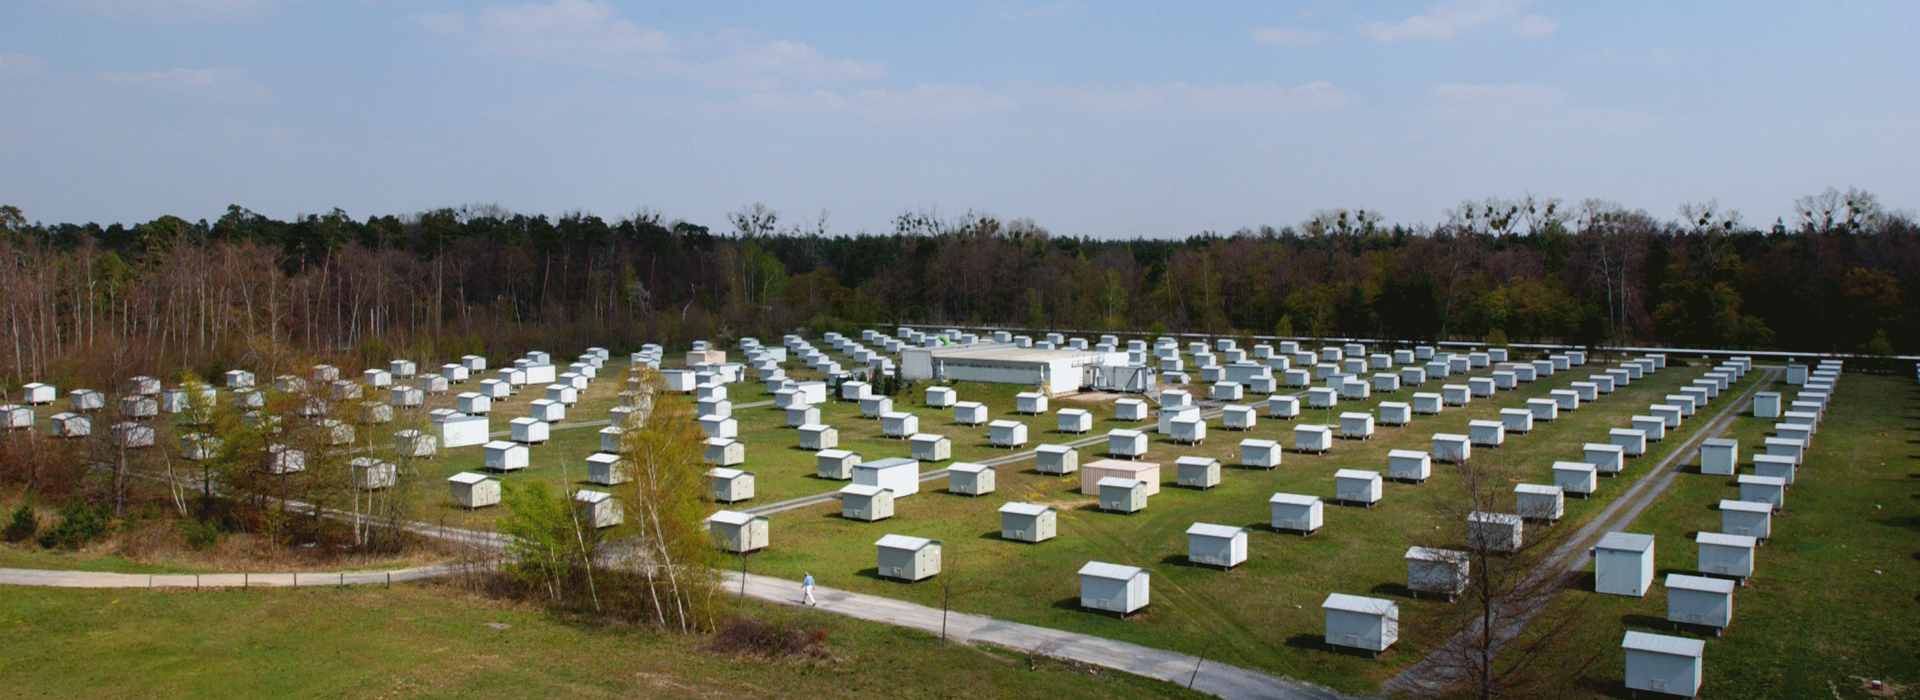
\includegraphics[width=0.6\textwidth]{img/kaskade.jpg}
    \caption{Foto del sito dove si trova KASKADE.}
    \label{img:kaskade}    
\end{figure}

Un altro meccanismo per la rivelazione dei raggi cosmici consiste nel principio di fluorescenza: le particelle cariche presenti negli sciami adronici e elettromagnetici interagiscono con l'azoto dell'atmosfera che transiscono in uno stato eccitato emettendo radiazione nel range $300-400\,\textup{nm}$, quando ritornano nel loro stato fondamentale. Questa radiazione, chiamata \emph{luce di fluorescenza} può attraversare kilometri di atmosfera senza essere assorbita. Per osservarla, come viene fatto nell'esperimento di Auger, si utilizzano dei telescopi: la luce viene raccolta da delle parabole, che la convogliano nel fuoco, dove si trova una matrice di PMT. Per questioni geometrice, ciascun PMT di questa matrice mappa una diversa regione dello spazio. Registrando dunque tempo di arrivo e altezza dell'impulso su ciascun PMT della matrice si riesce a ricostruire l'evoluzione dello sciame e l'energia della particella primaria.

Per completezza, un altro metodo con cui si rivelano i raggi cosmici è attraverso rivelatori di luce Cherenkov, sfruttando il fatto che l'aria si comporta come un mezzo con indice di rifrazione diverso da $1$. Le particelle relativistiche prodotte negli sciami infatti emettono luce Cherenkov, tipicamente una luce blu della durata di pochi $\textup{ns}$.

In alcuni casi è stato possibile effettuare misure di raggi cosmici dallo spazio, montando rivelatori di raggi cosmici su satelliti o stazioni orbitanti. Data la limitata disponibilità di spazio, è possibile osservare solo lo spettro delle basse energie, da confrontare poi con le misure ad alte energie compiute a terra. In questi casi, di esperimenti condotti nello spazio o su palloni, è possibile utilizzare campi magnetici (tipicamente prodotti da superconduttori) per poter discriminare il segno della carica delle particelle che passano dal rivelatore. Dalla misura di curvatura si determinano infatti il segno della carica e l'impulso della particella.

\section{Meccanismi di accelerazione dei raggi cosmici}\index{Accelerazione di raggi cosmici}

Partiamo da un semplice richiamo di un problema fondamentale, ovvero vogliamo studiare la curvatura di una particella carica nello spazio in presenza di un campo magnetico costante e uniforme $\vec{B}$. Partiamo scrivendo
\begin{gather}
    \frac{\der \vec{p}}{\der t} = \frac{Ze}{c}\vec{v} \times \vec{B} = m\frac{\der \gamma}{\der t}\vec{v} + m\gamma \frac{\der \vec{v}}{\der t} = m\gamma \frac{\der \vec{v}}{\der t}, \label{eq:RC1}\\
    \vec{p} = m\gamma \vec{v}. \notag
\end{gather}
Nel piano trasverso deve valere la seguente uguaglianza:
\begin{gather*}
    \biggl| \frac{\der \vec{v}}{\der t} \biggr| = \frac{v_\bot^2}{R},\\
    m\frac{v_\bot^2}{R} = \frac{Ze}{c}v_\bot B,
\end{gather*}
dove abbiamo sostiutito il risultato ottenuto in Eq.(\ref{eq:RC1}). Dunque otteniamo
\begin{equation}
    R = \frac{m\gamma v_\bot c}{ZeB} = \frac{pc}{Ze}\frac{\sin \theta}{B},
    \label{eq:RC2}
\end{equation}
\begin{definition}
    La variabile $R$ ricavata in Eq.(\ref{eq:RC2}) viene chiamata \emph{giroraggio}, mentre il rapporto $\displaystyle\frac{pc}{Ze}$ viene chiamato \emph{rigidità}, questa la si può intendere come la resistenza con cui la particella si oppone all'effetto di curvatura del campo magnetico. 
\end{definition}
\begin{notation}
    In molti testi si riporta con la lettera $R$ sia il giroraggio che la rigidità. Per evitare confusione utilizzeremo la seguente notazione:
    \begin{itemize}
        \item $R$ per il giroraggio,
        \item $\mathcal{R}$ per la rigidità.
    \end{itemize}
\end{notation}

Adesso vogliamo domandarci fino a che energie si possono misurare sui satelliti da una semplice misura di deflezione della traiettoria di una particella in campo magnetico. Il primo taglio, come già detto, è dovuto alla superficie finita disponibile sui satelliti, dunque risulta anche non producente utilizzare campi magnetici intensi a tal punto da curvare sensibilmente particelle che raramente osserveremo. Il secondo limite è imposto dalla risoluzione spaziale con cui riusciamo a misurare la curvatura della traiettoria. Si faccia riferimento alla figura Fig.(\ref{img:giroradius}).

\begin{figure}[H]
    \centering
    %\includegraphics[]{}
    \caption{Schematizzazione del problema.}
    \label{img:giroradius}
\end{figure}

Il campo magnetico presente nel rivelatore è di intensità $| \vec{B}| \sim 1\,\textup{T}$, la risoluzione spaziale è $\delta \sim 10 \,\mu\textup{m}$. La lunghezza del rivelatore lungo la quale la particella passa è di circa $L \sim 1\,\textup{m}$. Possiamo dunque misurare quanto la traiettoria della particella si discosta dalla  traiettoria rettilinea (\emph{sagitta} $s$), nel migliore dei casi misuriamo una distanza $\delta$:
\begin{gather}
    \begin{split}
        s & \sim R - R\cos \frac{\theta}{2} \sim R\frac{\theta^2}{8} \sim R \frac{L^2}{8 R^2}\\
               & \sim \frac{L^2}{8 R},\label{eq:giro1}
    \end{split}\\
    \delta s \sim \frac{L^2}{8}\frac{\delta R}{R^2}.\label{eq:giro2}
\end{gather}
In Eq.(\ref{eq:giro1}) abbiamo utilizzato il fatto che $\theta \ll 1$ e conseguentemente $\theta = L/R$. In Eq.(\ref{eq:giro2}) abbiamo utilizzato l'usuale propagazione degli errori. Da Eq.(\ref{eq:RC2}) notiamo che
\begin{equation*}
    \frac{\delta R}{R} = \frac{\delta p_\bot}{p_\bot},
\end{equation*}
dunque, sostituendo nell'equazione di prima otteniamo
\begin{equation*}
    \delta s = \frac{L^2 ZeB}{8p_\bot c} \frac{\delta p_\bot}{p_\bot},
\end{equation*}
se ad esempio imponiamo che $\delta p_\bot / p_\bot \sim 50\%$ otteniamo che
\begin{equation*}
    (p_\bot c)_\textup{max} = \frac{L^2 ZeB}{8\delta s} 0.5 = 3\,\textup{erg} \simeq 2\,\textup{TeV}. 
\end{equation*}
\begin{example}
    Chiediamoci dunque: un protone con energia di $\sim1\,\textup{TeV}$ quanto è influenzato dal campo magnetico solare? Supponiamo di voler calcolare la sagitta nella curvatura che il protone compie tra il sole e la terra (questo fissa la distanza $L$). Ricordiamo che $L_\textup{sole-terra} = 1\,\textup{UA} \sim 150\times 10^6\,\textup{km}$ e che $|\vec{B}|_\textup{sole} \sim 10\,\mu\textup{G}$. Usando Eq.(\ref{eq:RC2}) per ricavare $R$ e Eq.(\ref{eq:giro1}) per ricavare $s$ si ottiene
    \begin{equation*}
        s = \frac{L^2 ZeB}{8p_\bot c} \simeq 10^{-2}\,\textup{UA}.
    \end{equation*}
\end{example}
Consideriamo adesso la frequenza di rotazione in campo magnetico di una particella, possiamo scrivere la pulsazione come $\omega_\textup{G} = v_\bot / R$, dove $R$ è il giroraggio. Nel caso non relativistico e per carica unitaria possiamo portare avanti il calcolo come segue:
\begin{equation}
    \omega_\textup{G} = \frac{v_\bot}{mv_\bot c}eB = \frac{eB}{mc}. \label{eq:omegagiro}
\end{equation}
Se applichiamo un campo magnetico ad un atomo, questa formula descrive come cambia la frequenza di rotazione attorno al nucleo dell'elettrone. Di fatto corrisponde, se moltiplicato per $\hslash$, all'effetto Zeeman per l'atomo di idrogeno. Nella galassia è presente una grande quantità di idrogeno, osservabile perchè si vede una riga particolare che è quella a $1.4\,\textup{GHz}$ dell'idrogeno neutro. La frequenza di giroraggio risulta dunque essere $\nu_\textup{G} = 29\,\textup{GHz}/\textup{T}$. Dato che il campo magnetico solare è dell'ordine dei $10^{-9}\,\textup{T}$, otteniamo che la frequenza data dall'effetto Zeeman è $29\,\textup{Hz}$. Se modelliziamo l'elettrone classicamente, dunque in orbita intorno al nucleo, abbiamo che a seconda del verso di rotazione (orario o antiorario), il campo magnetico tende a far allontanare o avvicinare l'elettrone, dunque a rallentarlo o ad accelerarlo. Lo splitting di queste due popolazioni è di vitale importanza: conoscere la distanza tra i picchi delle due distribuzioni fornisce informazioni sul campo magnetico presente in quella regione di spazio.

Proviamo adesso a considerare un campo magnetico uniforme (nello spazio) e lentamente variabile, ($\Delta B / B$ piccolo) ovvero una variazione di campo magnetico piccola in un tempo prefissato, che è quello in cui la particella attraversa la regione dove è presente il campo magnetico ($T \simeq 1 / \nu_\textup{G}$). In queste condizioni possiamo considerare la traiettoria della particella come una spira percorsa da corrente, dunque possiamo considerare la corrente $i = Ze / T$. Ricordando Eq.(\ref{eq:omegagiro}), ricavando da questa l'espressione per la frequenza $\nu_\textup{G}$ e sostituendo l'espressione del giroraggio, calcoliamo il momento magnetico di questa spira:
\begin{gather}
    \nu_\textup{G} = \frac{v_\bot}{2\pi R}, \notag \\
    R = \frac{p_\bot c}{ZeB} = \frac{m v_\bot c}{ZeB} \notag \\
    \mu = \frac{iA}{c} = \frac{Ze v_\bot R}{2c} = \frac{1}{2}\frac{mv_\bot^2}{B} = \frac{W_\bot}{B}. \label{eq:mu_spira}
\end{gather}
dove con $W_\bot$ indichiamo l'energia cinetica trasversa. Ci chiediamo quanto vale la variazione del momento magnetico in un giro. Dunque analiziamo la variazione di $\Delta W$ in un giro. Ricordiamo che
\begin{equation*}
    \vec{\nabla} \times \vec{E} = -\frac{1}{c} \frac{\partial \vec{B}}{\partial t},
\end{equation*}
utilizzando le note relazioni tra campi vettoriali otteniamo che 
\begin{equation*}
    \int_{\delta S} \vec{E} \cdot \der \vec{l} = -\frac{1}{c} \int_{S} \frac{\partial \vec{B}}{\partial t},
\end{equation*}
dove con $\delta S$ intendiamo il contorno della superficie su cui integriamo. Il segno negativo davanti al secondo integrale si annulla con considerazioini date dalla regola della mano destra quando andiamo a calcolare il prodotto scalare presente nell'equazione. Utilizziamo l'approssimazione detta prima per il campo magnetico ed otteniamo
\begin{equation*}
    \int_{\delta S} \vec{E} \cdot \der \vec{l} = \frac{1}{c}\frac{\Delta B}{T} \pi R^2.
\end{equation*}
Per ottenere la variazione di energia cinetica scriviamo semplicemente
\begin{gather*}
    \Delta W_\bot = \frac{Ze \Delta B \pi R^2}{cT} = \frac{Ze \Delta B \pi R^2}{c} \frac{v_\bot}{2\pi R} = \frac{Ze\Delta B v_\bot}{2c} \frac{mv_\bot c}{ZeB} = \frac{\Delta B}{B} W_\bot,\\
    \frac{\Delta B}{B} = \frac{\Delta W_\bot}{W_\bot},
\end{gather*}
dove abbiamo sostituito l'espressione di $1/T$ con quella della frequenza di giroraggio, e abbiamo sostituito $R$ con Eq.(\ref{eq:giro2}). Ricordando adesso Eq.(\ref{eq:mu_spira}) otteniamo
\begin{equation*}
    \Delta \mu = \frac{\Delta W_\bot}{B} - W_\bot \frac{\Delta B}{B^2} = \frac{W_\bot}{B}\biggl(\frac{\Delta W_\bot}{W_\bot} - \frac{\Delta B}{B}\biggr) = 0,
\end{equation*}
possiamo dunque dire che $\mu$ in questo caso (campo magnetico lentamente variabile e particella non relativistica) è un invariante adiabatico. Ricaviamo quindi da Eq.(\ref{eq:mu_spira})
\begin{equation}  
    \begin{cases}
        \Delta \biggl(\displaystyle\frac{p_\bot^2}{B}\biggr) = 0, \\
        \Delta (BR^2) = 0,
    \end{cases}
    \label{eq:adiabatico}
\end{equation}
dove l'ultima espressione è stata ottenuta facendo una sostituzione con l'espressione del giroraggio, dalla quale abbiamo ricavato l'espressione per $p_\bot$. In particolare, questa ultima espressione ci dice che l'integrale sull'area del campo magnetico è costante.

\begin{example}[Fasce di Van Allen]
    Il campo magnetico terrestre è un campo magnetico di dipolo, dunque con un addensamento di linee di campo in prossimità dei poli. Se una particella carica a bassa energia arriva in prossimità del campo magnetico terrestre, considerando che localmente possiamo approssimare il campo magnetico terrestre come uniforme, sappiamo che il moto a cui sarà soggetta la particella è di tipo elicoidale. Ricordando la coppia di equazioni Eq.(\ref{eq:adiabatico}), possiamo concludere che in questa prima fase di traiettoria della particella, il raggio dell'elica sarà costante. La particella dunque continua a seguire la linea di campo di $\vec{B}$. Quando la particella procede con la sua traiettoria nella regione più vicina ai poli, dove il campo magnetico si intensifica, se $B$ aumenta, $R$ diminuisce (con $\sqrt{B}$), inoltre sempre da Eq.(\ref{eq:adiabatico}) deve aumentare l'energia cinetica trasversa. Dato che la forza di Lorentz non fa lavoro possiamo scrivere
    \begin{equation*}
        \vec{F} \cdot \vec{v} = 0,
    \end{equation*}
    dunque
    \begin{equation*}
        \sqrt{p_\bot^2 c^2 + p_\parallel ^2 c^2 + m^2 c^4} = \textup{costante}.
    \end{equation*}
    Dovendosi conservare il rapporto $p_\bot^2 / B$ possiamo affermare che la velocità di rotazione attorno alla linea di campo aumenta, diminuisce invece la componente parallela (dovendosi conservare $W$). Scrivendo la relazione 
    \begin{equation*}
        \vec{F} = - \vec{\nabla} (\vec{\mu} \cdot \vec{B})
    \end{equation*}
    si nota subito che se $B$ aumenta, la forza lo respinge e viceversa. Dunque quando la particella si avvicina al polo non solo inizia a girare più velocemente ma ad un certo punto cambia pure direzione. Il comportamento di nostro interesse è infatti quello per cui una particella, quando arriva in una zona con forti campi magnetici, rimbalza. Potremmo dare il nome di \emph{specchi magnetici} a questi tipi di effetti, utilizzati ad esempio per il confinamento di plasmi.
\end{example}

\subsection{Meccanismo di accelerazione di Fermi}
Il primo meccanismo di accelerazione che studiamo è una semplificazione di quello proposto da Enrico Fermi nel 1949. Una particella ultrarelativistica di carica $Ze$ si muove con impulso $\vec{p}$ verso un fronte d'onda di una nube di campo magnetico $\vec{B}$, questa ha una velocità $\vec{v}$, senza perdita di generalità supponiamo $\vec{v}$ diretta lungo la direzione positiva dell'asse $\hat{z}$ e $\vec{p}\cdot\hat{z} < 0$, dunque siamo nello scenario in cui nube magnetica e particella si stanno avvicinando con un certo angolo di inclinazione $\theta$ relativo tra i due. Consideriamo inoltre che la massa della nube sia molto maggiore di quella della particella. Nel sistema di riferimento in quiete con la nube, l'urto tra nube e particella è di tipo elastico, si conserva cioè la componente dell'impulso $\vec{p}_\parallel '$ parallela alla superficie della nube. 

Facendo una trasformazione di Lorentz nel sistema di riferimento in quiete con la nube, possiamo scrivere
\begin{gather*}
    E_i' = \gamma_v (E_i + c\beta_v p_{z, i}),\\
    cp_{z, i}' = \gamma_v (cp_{z, i} + \beta_v E_i),
\end{gather*}
dove con il pedice $v$ si intende il valore di velocità della nube, ricordando che stiamo facendo un boost nel sistema di riferimento della nube, con il pedice $i$ si intende la quantità iniziale. Quello che vogliamo imporre è
\begin{gather*}
    E_f' = E_i',\\
    p_{z, f}' = - p_{z, i}'.
\end{gather*}
Siamo interessati all'energia finale della particella nel sistema di riferimento del laboratorio:
\begin{equation*}
    \begin{split}
        E_{f} & = \gamma_v (E_{f}' - c\beta_v p_{z,i}') = \gamma_v (E_i' + c\beta_v p_{z,i}')\\
              & = \gamma_v (\gamma_v (E_i + c\beta_v p_{z,i}) + \beta_v \gamma_v (cp_{z, i} + \beta_v E_i))\\
              & = \gamma_v^2 E_i + 2 \gamma_v^2 \beta_v c p_{z, i} + \gamma_v^2 \beta_v^2 E_i \\
              & = \gamma_v^2 (E_i + 2 \beta_v c p_{z, i} + \beta_v^2 E_i) \\
              & \simeq (1+\beta_v^2 ) (\cdots),
    \end{split}
\end{equation*}
esplicitando i calcoli per $E_f - E_i$, lasciando solo i termini al primo ordine in $\beta_v^2$, otteniamo che
\begin{equation}
    \frac{\Delta E}{E} = 2 \beta_v^2 + 2 \beta_v \frac{p_ic}{E}\cos \theta \simeq 2 (\beta_v^2 + \beta_v \cos \theta). \label{eq:betavcoshtheta}
\end{equation}
dove abbiamo utilizzato il fatto che $p_i c / E = \beta \simeq 1$. Aggiungiamo adesso la complicazione che i fronti d'onda che la particella incontrerà saranno in numero maggiore di 1, consideriamo per il momento che il passo tra un fronte e il successivo sia $\lambda$. Se le velocità della particella e delle nubi sono $\vec{v}$ e $\vec{V}$ con un angolo relativo $\theta$, possiamo scrivere che la velocità realtiva è
\begin{equation*}
    v_\textup{rel} = \frac{v\cos \theta + V}{1 + \frac{vV}{c^2}\cos \theta},
\end{equation*}
se le due velocità sono concordi invece
\begin{equation*}
    v_\textup{rel} = \frac{v\cos \theta - V}{1 - \frac{vV}{c^2}\cos \theta}.
\end{equation*}
Se approssimiamo la prima delle due in $V/c$, proprio come prima abbiamo fatto con $\beta_v$, otteniamo
\begin{equation}
    \begin{split}
        v_\textup{rel} & \simeq (v\cos \theta + V)\biggl(1 - \frac{vV}{c^2} \cos \theta \biggr) = v \cos \theta + V \sin^2 \theta \label{eq:thetaaverage} \\
                       & \simeq 
                        \begin{cases}
                            c (\cos \theta + \frac{V}{c} \sin^2 \theta), \quad \cos \theta > 0 \\
                            - c (\cos \theta - \frac{V}{c} \sin^2 \theta), \quad \cos \theta < 0
                        \end{cases}
    \end{split}
\end{equation}
Adesso dunque vogliamo mediare Eq.(\ref{eq:betavcoshtheta}) sulla funzione di $\cos\theta$ di Eq.(\ref{eq:thetaaverage}). Faccio dunque il valore di aspettazione, normalizzando per la funzione distribuzione di $\theta$
\begin{equation*}
    \mathbb{E}\biggl[\frac{\Delta E}{E}\biggr] = \frac{\int_{-1}^{+1}\frac{\Delta E}{E} v_\textup{rel}(\cos \theta) \der \cos \theta}{\int_{-1}^{+1}v_\textup{rel}(\cos \theta) \der \cos \theta} = \frac{V}{c} = \beta_v.
\end{equation*}
Abbiamo ottenuto il risultato integrando correttamente sulle diverse regioni di $v_\textup{rel}$, usando inoltre la parità/disparità dei vari termini si velocizzano i calcoli. Dunque abbiamo ottenuto che $\Delta E / E \simeq 3 \beta_v^2 \equiv \xi $, dopo un rimbalzo la particella ha energia $E_1 = E_0 (1 + \xi)$, dopo $n$ rimbalzi ha energia $E_n = E_0 (1 + \xi)^n$. Siamo adesso interessati a calcolare la probabilità che una particella con una certa energia iniziale $E_0$ raggiunga una energia fissata $\overline{E}$. Iniziamo osservando che 
\begin{equation}
    \overline{n} = \frac{\ln \overline{E} / E}{\ln (1+ \xi)},\label{eq:overline_n}
\end{equation}
dunque dobbiamo chiederci quanto valga la probabilità che la particella riesca a fare più di $\overline{n}$ rimbalzi. Data la probabilità di fuga $p_\textup{F}$, la probabilità di rimanere intrappolata nel meccanismo di accelerazione per $n$ volte varrà $(1 - p_\textup{F})^n$. Ricollegandoci alla domanda precedente, siamo ora interessati a calcolare la probabilità 
\begin{equation*}
    \Pr (E > \overline{E}) = \sum_{i = \overline{n}} ^{\infty} (1 - p_\textup{F})^i = \frac{(1 - p_\textup{F})^{\overline{n}}}{p_\textup{F}},
\end{equation*}
dove abbiamo utilizzato la proprietà della serie geometrica per ricavare il risultato finale. Se moltiplichiamo questa quantità per il numero inziale di particelle otteniamo una stima di quante particelle hanno almeno energia $\overline{E}$
\begin{equation*}
    \textup{N} (E > \overline{E}) = \alpha \frac{(1 - p_\textup{F})^{\overline{n}}}{p_\textup{F}},
\end{equation*}
se adesso sostituiamo l'espressione di $\overline{n}$ di Eq.(\ref{eq:overline_n}) e ricaviamo nuovamente $\textup{N}$, otteniamo
\begin{equation*}
    \textup{N} (E > \overline{E}) = D \biggl(\frac{\overline{E}}{E}\biggr)^{\ln(1 - p_\textup{F}) / \ln (1 + \xi)} \equiv D \biggl(\frac{\overline{E}}{E}\biggr) ^ {-\gamma},
\end{equation*}
Dove $D$ tiene di conto di tutte le costanti moltiplicative e $\gamma$ è un fattore all'esponente. Derivando questra equazione otteniamo la forma 
\begin{equation}
    \frac{\der N}{\der E} \varpropto E^{- (\gamma + 1)}.\label{eq:gammaplusone}
\end{equation}
Riguardo $\gamma$ possiamo dire
\begin{equation*}
    \gamma = \frac{\ln(1 - p_\textup{F})}{\ln ( 1 + \xi)} \simeq \frac{p_\textup{F}}{\xi},
\end{equation*}
dovremmo quindi confrontare l'espressione dell'esponente in Eq.(\ref{eq:gammaplusone}) con il valore sperimentale osservato ($\simeq 2.7$), riguardante Fig.(\ref{img:cosmicrays}), dunque imporremo $\gamma \simeq 1.7$. Si ricava quindi un valore approssimato per la probabilità di fuga $p_\textup{F} \simeq \gamma / \xi \simeq 1.7 \cdot 3 \times 10^{-8} = 5.1 \times 10^{-8}$. Qundi per arrivare ad energia $\overline{E}$ deve fare, con i valori di $\xi = 3 \times 10^{-8}$ e $\overline{E} = 1\,\textup{TeV}$, $\overline{n} \simeq 4 \times 10^{8}$ rimbalzi. Per capire se questo processo è possibile o meno, ricordiamo che nelle ipotesi iniziali del problema abbiamo detto che i fronti d'onda distano $\lambda$ l'uno dal successivo e che la velocità della nostra particella è $\sim c$, dunque possiamo dare una stima della distanza percorsa dalla particella prima di raggiungere l'energia $\overline{E}$. Prima di fare ciò occorre capire quanto vale $\lambda$: le sorgenti di questi tipi di fenomeni sono tipicamente i residui di supernova, che hanno dimensioni tipiche del \emph{parsec} (circa $3$ anni-luce). Dunque per far avvenire un processo di accelerazione possiamo calcolare $t_\textup{acc} = \lambda / c \simeq 3\,\textup{years}$, il tempo necessario totale sarà $t_\textup{tot} = t_\textup{acc} \cdot \overline{n} = 1.2\times10^{9}\,\textup{years}$.
Una delle caratteristiche misurabili dei raggi cosmici è la composizione isotopica, ad esempio del $^{10}\textup{Be}$, con una vita media di $10^6\,\textup{years}$. Se ne misura la composizione isotopica in relazione con gli altri isotopi, e osserviamo che, essendo in grado di conoscerne la percentuale nel punto di produzione, posso misurare la composizione in un secondo momento per stimare il tempo trascorso. Dalle nostre misure sulla percentuale di $^{10}\textup{Be}$ si stima che il tempo di percorrenza sia $10^7\,\textup{years}$, quindi la stima ricavata prima di $t_\textup{tot}$ risulta errata poichè incompatibile con la vita media dell'isotopo stesso.
Il fattore che fa aumentare $\overline{n}$ nel nostro caso è la dipendenza al denominatore di $\beta_v^2$.

\section{Meccanismo di accelerazione di shock}
Il meccanismo di accelerazione di Fermi presenta due inconvenienti: c'è una dipendenza al numeratore da $\beta_v^2$ e non è nota a priori la probabilità di fuga $p_\textup{F}$. In questo nuovo caso consideriamo un'onda d'urto di shock, lo facciamo nel caso monodimensionale, fronte d'onda piano infinito, che si propaga in un mezzo (ad esempio gas di protoni) con una velocità $\vec{u}$ molto superiore alla velocità del suono nel mezzo $c_\textup{s}$. Il fronte d'urto supponiamo si muova verso destra, dividiamo lo spazio in due zone: la prima a valle del fronte d'urto, la seconda a monte del fronte d'urto. Ci mettiamo nel sistema di riferimento solidale con il fronte d'onda, quindi la porzione di spazio a valle del fronte d'onda si avvicina con velocità $v_1 = u$, il gas a monte ha velocità $v_2$. Le due parti di spazio hanno inoltre rispettivamente le grandezze $\rho_1$, $T_1$ e $p_1$, $\rho_2$, $T_2$ e $p_2$. Nell'attraversamento del fronte d'onda di shock vogliamo imporre la conservazione delle grandezze di massa, impulso ed energia del fluido di protoni.

Data l'assenza di alcuna fonte di materia, impulso o di energia abbiamo
\begin{gather}
    \rho_1 v_1 = \rho_2 v_2,\notag \\
    p_1 + \rho_1 v_1^2 = p_2 + \rho_2 v_2^2, \label{eq:cont2shock}\\
    \rho_1 v_1 \biggl( \frac{1}{2}v_1^2 + h_1 \biggr) = \rho_2 v_2 \biggl( \frac{1}{2}v_2^2 + h_2 \biggr).\label{eq:cont3shock}
\end{gather}
Dagli approfondimenti trattati in App.(\ref{chap:app1}), possiamo semplificare questo sistema scrivendo che
\begin{equation*}
    \begin{cases}
        \displaystyle h = \epsilon + pV = \mu c_\textup{v} T + pV= \frac{c_\textup{v}}{c_\textup{p} + \textup{v}} pV + pV = pV \frac{\gamma}{\gamma - 1}\\
        pV = \mu R T 
    \end{cases},
\end{equation*}
inoltre posso scrivere che 
\begin{equation*}
    v = \frac{\textup{cost}}{\rho} \equiv J V,
\end{equation*}
dopo alcune sostituzioni otteniamo che Eq.(\ref{eq:cont2shock}) ci permette di ricavare il valore di $J$
\begin{equation*}
    J^2 = \frac{p_1 - p_2}{V_2 - V_1}.
\end{equation*}
Eq.(\ref{eq:cont3shock}) ci permette invece di scrivere
\begin{equation*}
    h_1 - h_2 = -\frac{1}{2}J^2(V_1^2 - V_2^2),
\end{equation*}
possiamo sostituire ad $h$ e $J^2$ le espressioni ricavate prima ed ottenere
\begin{equation*}
    \frac{\gamma}{\gamma - 1} (p_1 V_1 - p_2 V_2) + \frac{1}{2}(p_1 - p_2)(V_1 + V_2) = 0.
\end{equation*}
Possiamo dunque ricavarici il seguente rapporto
\begin{equation}
    \frac{V_2}{V_1} = \frac{(\gamma + 1)p_1 + (\gamma - 1)p_2}{(\gamma + 1)p_2 + (\gamma - 1)p_1},\label{eq:V2fracV1}
\end{equation}
sostituendo nell'espressione di $J^2$ questo rapporto otteniamo
\begin{equation*}
    J^2 = \frac{(\gamma + 1)p_2 + (\gamma - 1)p_1}{2V_1}.
\end{equation*}
Possiamo adesso scrivere l'espressione di $v_1^2$
\begin{equation}
    v_1^2 = J^2 V_1^2 = \frac{V_1}{2}\bigl[ (\gamma + 1)p_2 + (\gamma - 1)p_1 \bigr].\label{eq:v_1^2}
\end{equation}
\begin{definition}[Numero di Mach]
    Il rapporto tra la velocità $v$ di un oggetto nel fluido e la velocità del suono $c_\textup{s}$ nel fluido è chiamato \emph{numero di Mach}
    \begin{equation*}
        M \equiv \frac{v}{c_\textup{s}}
    \end{equation*}    
\end{definition}
In App.(\ref{chap:app1}) abbiamo trovato che 
\begin{equation*}
    c_{\textup{s}, i} = \sqrt{\gamma \frac{p_i}{\rho_i}}
\end{equation*}
per il fluido $i$-esimo. Nel nostro caso abbiamo
\begin{equation*}
    M_1^2 = \frac{v_1^2}{\gamma p_1 V_1},
\end{equation*}
in Eq.(\ref{eq:v_1^2}) abbiamo ricavato l'espressione per $v_1^2$, possiamo sostituire ed ottenere
\begin{equation*}
    M_1^2 = \frac{(\gamma + 1)p_2 + (\gamma - 1)p_1}{2 \gamma p_1},
\end{equation*}
si nota dunque che possiamo scrivere il numero di Mach come funzione unicamente del rapporto tra le pressioni a valle e a monte del fronte d'onda di shock
\begin{equation*}
    \frac{p_2}{p_1} = \frac{2 \gamma M_1^2 - (\gamma - 1)}{\gamma + 1}.
\end{equation*}
Si nota ad esempio che se $M$ tende a $+\infty$, si ha che la pressione nella zona a monte è molto maggiore di quella a valle.

Vogliamo invece trattare adesso il caso analogo ma per le desità e le velocità. Consideriamo ad esempio 
\begin{equation*}
    \frac{\rho_2}{\rho_1} = \frac{V_1}{V_2} = \frac{v_1}{v_2} = \frac{1 + \gamma}{(\gamma - 1) + \frac{2}{M_1^2}},
\end{equation*}
dove al terzo passaggio abbiamo sfruttato la conscenza del rapporto $p_2 / p_1$ e la relazione di Eq.(\ref{eq:V2fracV1}). In questo caso, se $M_1^2$ tende a $+\infty$ abbiamo che $V_1/V_2$ tende a un rapporto finito $(\gamma + 1) / (\gamma - 1)$, che per il gas di protoni (monoatomico) vale $4$. Abbiamo quindi trovato che in caso ultrasonico, la velocità nella zona a monte vale $v_2 = u/4$ . È possibile verificare sperimentalmente questi dati osservando i residui di supernovae. Inoltre, nello stesso limite per $M_1^2$ possiamo scrivere
\begin{equation*}
    \frac{T_2}{T_1} = \frac{p_2V_2}{p_1V_1} \varpropto M_1^2
\end{equation*}

Consideriamo il sistema di riferimento solidale con il gas di protoni a valle del fronte d'urto. Il fronte d'urto si muove verso destra con velocità $\vec{u}$. Il gas che si trova a monte si muove verso destra con velocità $\frac{3}{4}\vec{u}$, per convincersi basti pensare che la velocità relativa è $\frac{3}{4}u$. Poniamoci nel punto di vista della particella a valle che passando il fronte d'urto si ritrova nella zona a monte. Supponiamo che l'interazione avvenga con il campo magnetico. La particella che segue questa successione di eventi si ritrova nella parte a monte, dove la velocità del fluido è $\frac{3}{4}\vec{u}$. Dal punto di vista della parte a monte, la parte a valle si dirige verso la parte a monte con velocità $-\frac{3}{4}\vec{u}$, vedendosi arrivare addosso una nube elettromagnetica. In generale può avvenire lo stesso meccanismo di attraversamento del fronte d'urto. Dunque, che la particella si trovi a monte o a valle, si vede in ogni caso avvicinare la frazione di spazio complementare con velocità $\mp\frac{3}{4}\vec{u}$. L'attraversamento del fronte d'urto può in effetti avvenire più di una volta e quello che vogliamo fare adesso è calcolare il guadagno di energia per ogni attraversamento. L'unica accortezza da tenere è che nel caso del sistema di riferimento solidale con la parte a monte, la velocità del fronte d'urto vale $\frac{1}{4}\vec{u}$.

Poniamo dunque che la particella si trovi nella parte a valle. L'energia della particella nel sistema di riferimento della nube che si trova a monte vale
\begin{equation*}
    E' = \gamma_v(E + \beta_v pc \cos \theta),
\end{equation*}
dove $\theta$ è l'angolo relativo tra $\vec{p}$ (impulso della particella) e $\vec{u}$. Rinunciamo all'ipotesi di rimbalzo elastico: la particella viene infatti isotropizzata nella parte a monte e l'angolo di emissione sarà in generale diverso da $\theta$. Approssimando al primo ordine in $\beta_v$ possiamo scrivere $\gamma_v \sim 1$. Ricaviamo immediatamente che 
\begin{equation*}
    \frac{\Delta E}{E} \simeq \beta_v \frac{pc}{E} \cos \theta \simeq \beta_v \cos \theta.
\end{equation*}
Vogliamo dunque ricavare la probabilità che la particella, vada ad urtare contro la superficie. Per fare ciò notiamo che il risultato è semplicemente dato dal numero di particelle che sono contenute nel cilindro che interseca la superficie del fronte d'urto
\begin{equation*}
    N = n c \cos \theta s \Delta t,
\end{equation*}
dove $n$ è la densità del fluido, $c$ la velocità della particella dato che siamo in approssimazione ultrarelativistica e $s$ è la superficie che interseca il cilindro che ho considerato. Per ottenere la probabilità basterà mediare la funzione di prima con questa distribuzione, opportunamente normalizzata
\begin{equation*}
    \displaystyle\Pr(\textup{attraversamento}) \varpropto \frac{\displaystyle\int_0^{\frac{\pi}{2}}\cos^2 \theta \der \cos \theta}{\displaystyle\int_0^{\frac{\pi}{2}}\cos \theta \der \cos \theta} = \frac{2}{3}.
\end{equation*}
Si noti che la differenza sostanziale con il meccanismo di Fermi è che in questo caso non abbiamo supposto una successione di fronti d'urto a distanza $\lambda$, in questo nuovo meccanismo (capito intorno agli anni '70) le particelle attraversano più volte lo stesso fronte d'urto. Se la particella attraversa doppiamente il fronte d'urto (dunque dalla parte a valle si ritrova nuovamente nella parte a valle) abbiamo che
\begin{equation*}
    \frac{\Delta E}{E} = 2 \frac{2}{3} \beta_v = \frac{4}{3}\beta_v = \frac{4}{3}\frac{3}{4}\frac{u}{c} \equiv \xi,
\end{equation*}
infatti il calcolo che andrebbe fatto per l'attraversamento da zona a monte a zona a valle è in questo caso perfettamente simmetrico al calcolo fatto per l'attraversamento da valle a monte, questo spiega il fattore $2$ nell'ultima espressione. Con questo meccanismo è inoltre possibile calcolarsi la probabilità di fuga $p_\textup{F}$. Per impostare il calcolo si noti che 
\begin{itemize}
    \item mentre la particella si trova a valle, questa si vede arrivare il fronte d'urto a velocità $\vec{u}$, attraverserà sicuramente il fronte,
    \item mentre la particella si trova a monte, il fronte si allontana con velocità $\frac{1}{4}\vec{u}$. 
\end{itemize}
Bisogna considerare il flusso delle particelle del secondo caso
\begin{equation*}
    n \int_0^{\frac{\pi}{2}} \frac{c\cos \theta der \Omega}{4\pi} = \frac{nc}{4} \equiv J_\textup{p},
\end{equation*}
questo è il flusso $J$ che urtano sulla superficie. Il flusso di particelle che fuggono sarà invece $\frac{nu}{4}$, dunque la probabilità di continuare a sbattere contro il fronte d'urto vale 
\begin{equation*}
    \Pr = \frac{nc / 4}{(nc/4) + (nu/4)} = \simeq 1 - \frac{u}{c},
\end{equation*}
dunque la probabilità di fuga è $u/c$, svolgendo calcoli simili a quelli del meccanismo di Fermi otteniamo che
\begin{equation*}
    \frac{\der N}{\der E} \varpropto E^{-2}.
\end{equation*}

\section{I luoghi di accelerazione nell'universo}
In Fig.(\ref{img:snr}) si osservano alcune foto di residui di supernovae dove si pensa che abbia luogo il meccanismo di accelerazione di raggi cosmici.
\begin{figure}[H]
    \centering
    \subfloat[\centering SN 1542]{{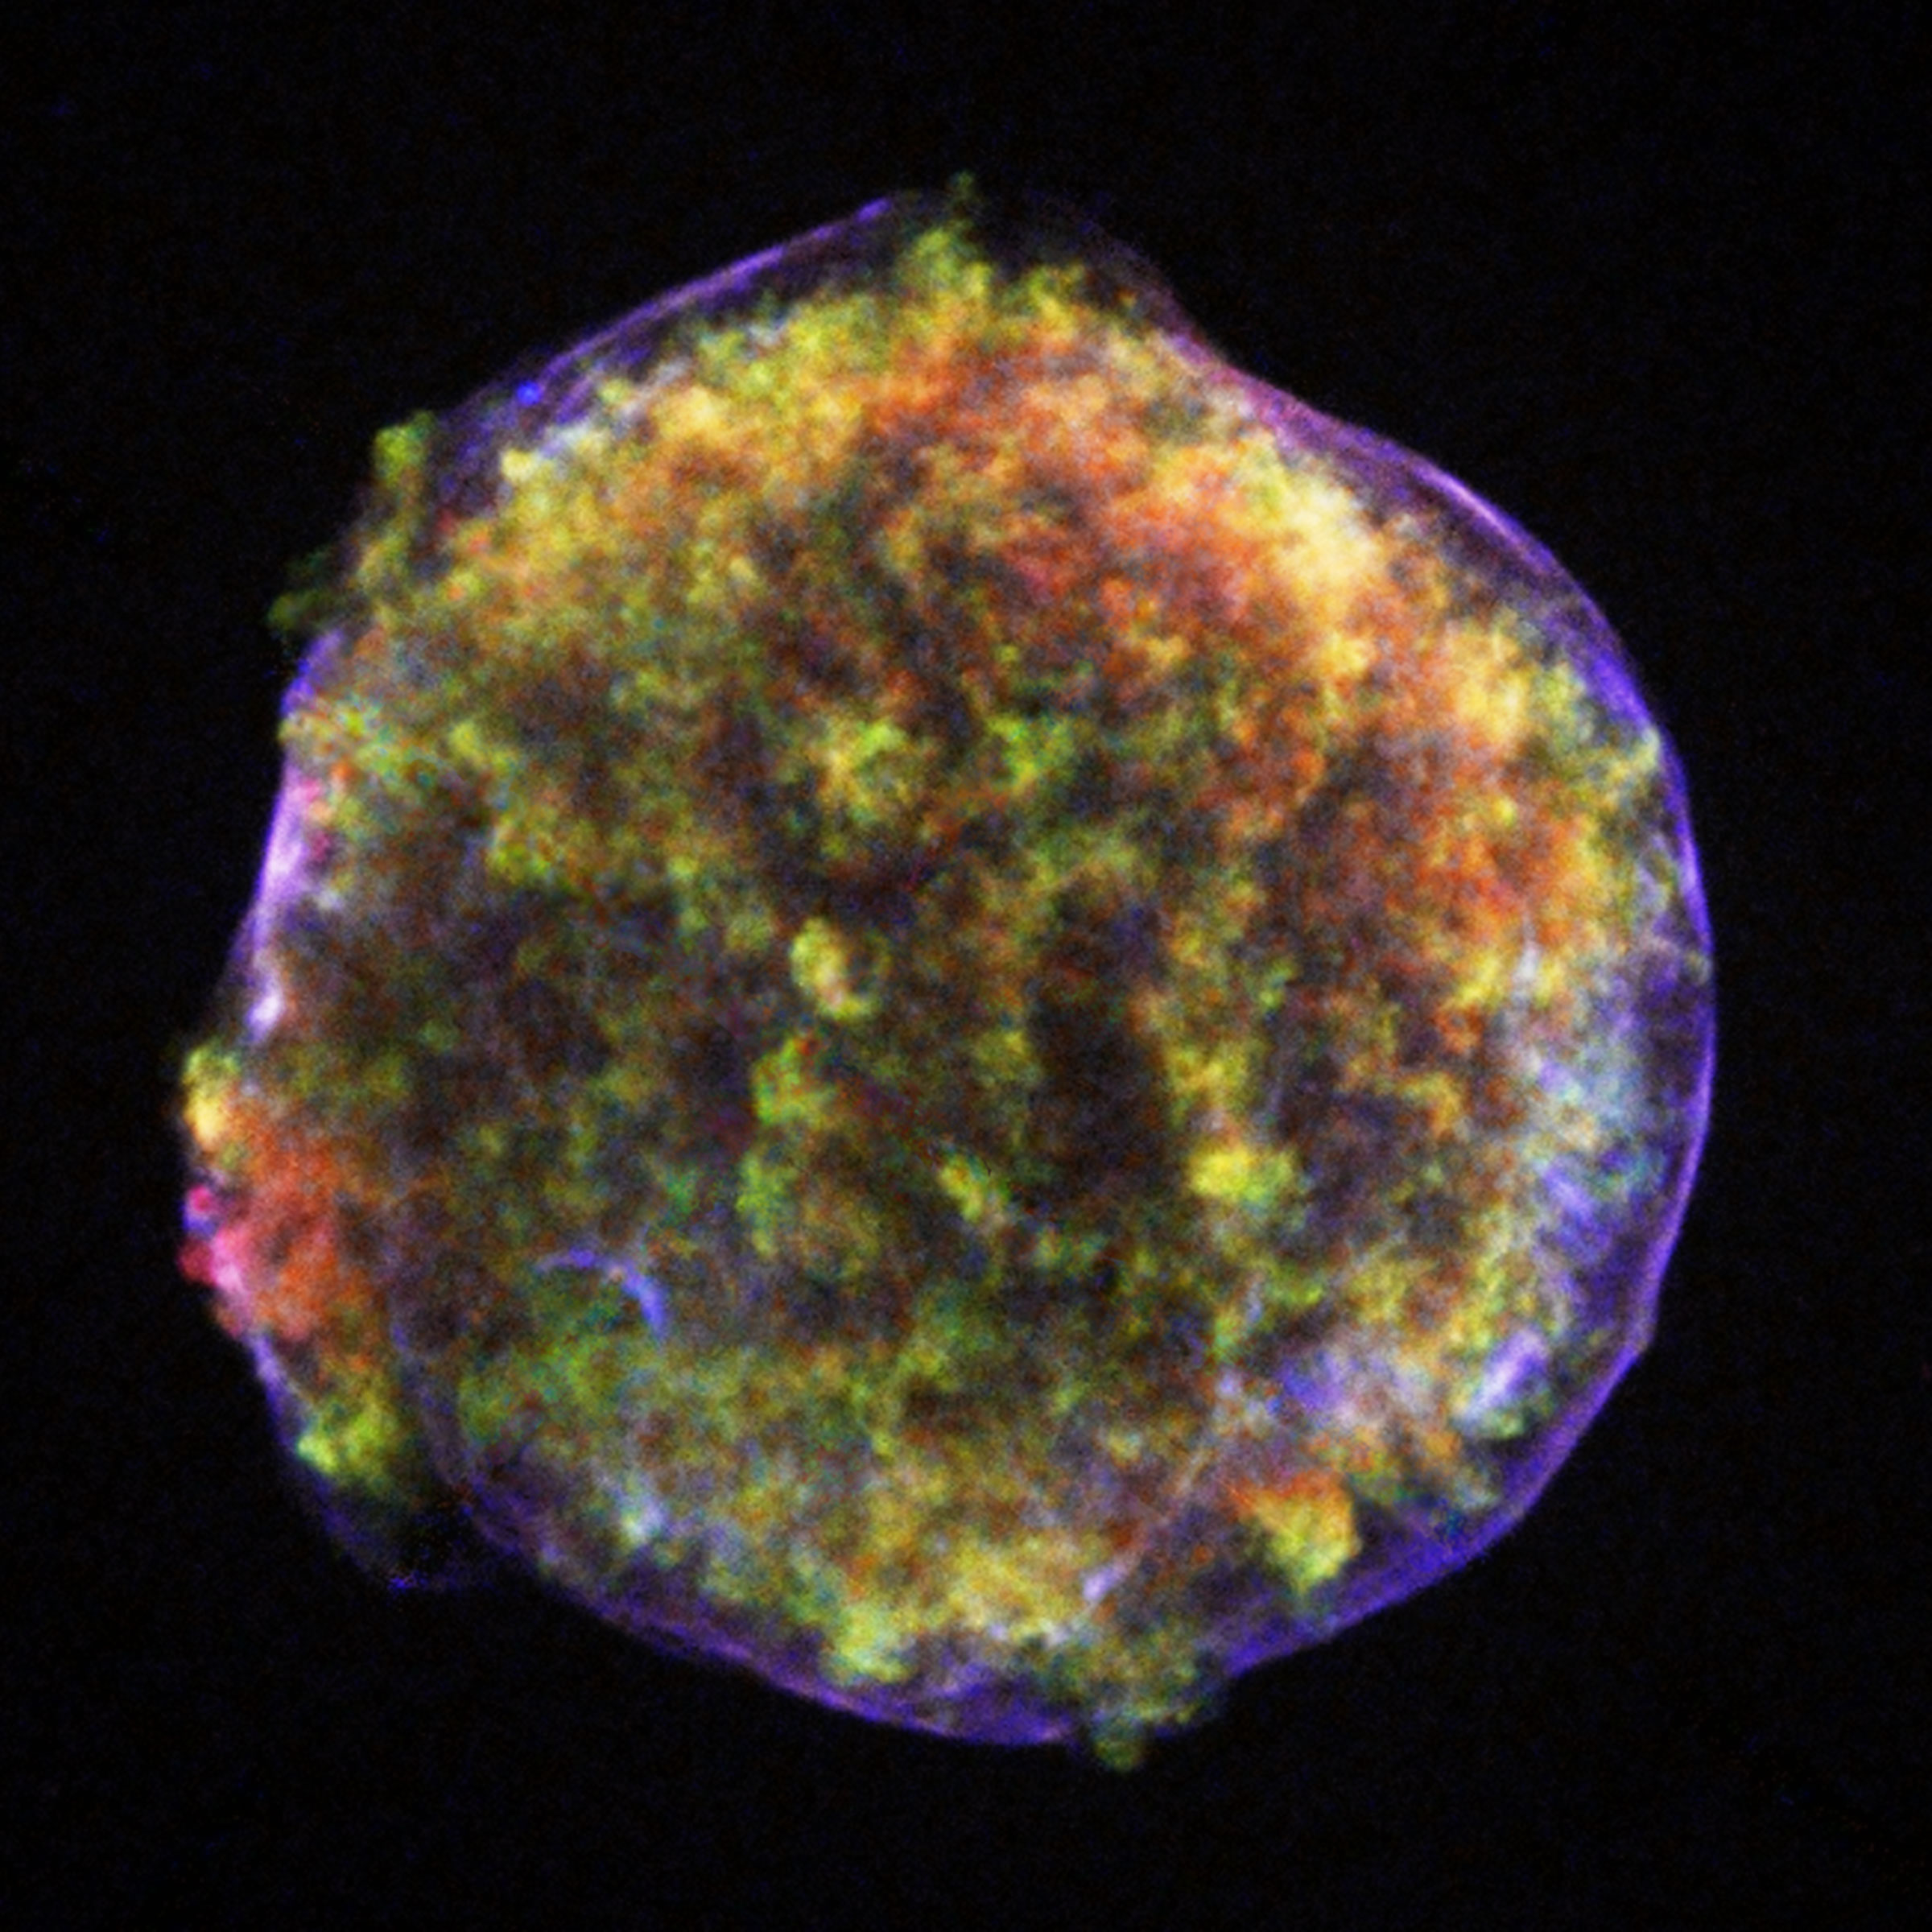
\includegraphics[width=0.3\textwidth]{img/Tycho-supernova-xray.jpg}}}%
    \quad
    \subfloat[\centering Nebulosa del Granchio]{{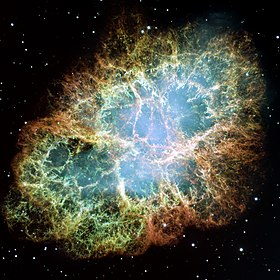
\includegraphics[width=0.3\textwidth]{img/Crab_Nebula.jpg}}}%
    \caption{A sinistra immagine ai raggi X della supernova Tycho, a distanza di $10\,\textup{k a.l.}$, di tipo Ia. A destra immagine nello spettro visibile della Nebulosa del Granchio (1052), a distanza di $6\,\textup{k a.l.}$, di tipo II.}%
    \label{img:snr}    
\end{figure}
Questi, come altri esempi (vedi la nebulosa Keplero 1604), sono appunto solo ipotizzati essere i centri di accelerazione dei raggi cosmici. L'unico modo per avere una certezza consiste nell'osservare raggi cosmici provenienti direttamente da questi siti, ma data la presenza di un campo magnetico non nullo nella galassia questi sarebbero sicuramente deviati. L'obiettivo dunque è quello di osservare particelle neutre provenienti da questi siti, in quanto non soggette a forza di Lorentz. Dato che, come abbiamo accennato, in questi luoghi c'è un'alta concentrazione di protoni, la speranza è di avere in seguito ad un urto la produzione di $\pi^0$ che, decadendo elettromagneticamente, dà origine a due fotoni. L'osservazione di questi fotoni può dunque darci informazione sui meccanismi di accelerazione e sui siti dove questi meccanismi hanno luogo. L'esperimento di FermiLAT ha misurato lo spettro in energia dei fotoni provenienti dai residui di supernova.
\subsection{Altri meccanismi di accelerazione}
Oltre ai residui di supernova, si ipotizza che ci siano altri meccanismi di accelerazione dei raggi cosmici:
\begin{itemize}
    \item pulsar, scoperte nel 1967,
    \item stelle di neutroni, che hanno campi magnetici intensi.
\end{itemize}

\subsubsection*{Argomento di Syrovatskii}
Se consideriamo una pulsar in rapida rotazione, questa può essere modellizzata come una spira di lato $L$, con un campo magnetico rotante di intensità $B$. Come sappiamo dalle equazioni di Maxwell, una variazione di campo magnetico dà origine ad un campo elettrico. Schematizzando il problema come in Fig.(\ref{img:syro}), possiamo scrivere la seguente equazione
\begin{equation*}
    \vec{\nabla} \wedge \vec{E} = - \frac{1}{c}\frac{\partial \vec{B}}{\partial t},
\end{equation*}
data la schematizzazione del problema possiamo semplificare come seguente
\begin{equation*}
    4 \overline{E} L = \frac{1}{c} \frac{\Delta B}{\Delta t} L^2 = \frac{\omega}{c} B L^2.
\end{equation*}
Possiamo dunque ricavare il massimo valore del lavoro che può essere compiuto su una particella di carica $e$
\begin{equation*}
    \epsilon_\textup{MAX} = e \overline{E} L = \frac{eBL}{4} = \textup{O}(10^{20}\,\textup{eV}).
\end{equation*}

\begin{figure}[H]
    \centering
    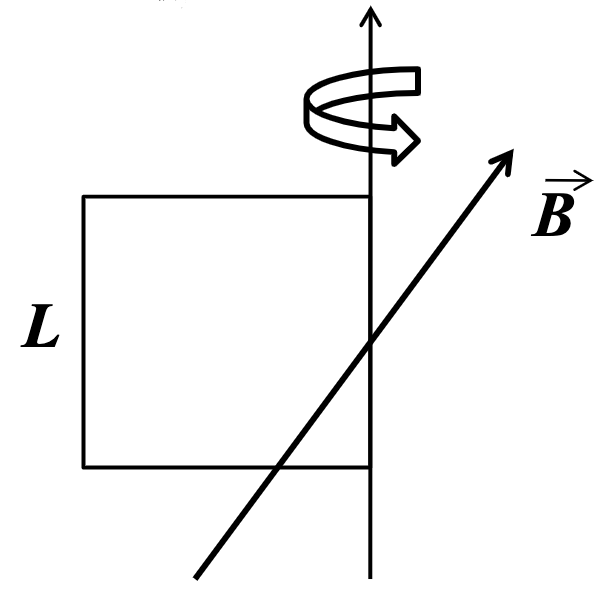
\includegraphics[width=0.4\textwidth]{img/syro.png}
    \caption{Schematizzazione del problema.}
    \label{img:syro}    
\end{figure}

\section{Taglio GZK}

Abbiamo visto che ad alte energie lo spettro in energia dei raggi cosmici ha una incurvatura. Per spiegare questo fenomeno è stato ipotizzato che le particelle cariche ad alta energia interagiscano con la radiazione cosmica di fondo con un processo di produzione di soglia di questo tipo
\begin{equation*}
    p + \gamma \rightarrow \Delta^+ \rightarrow N + \pi.
\end{equation*}
La particella $\Delta^+$ è una risonanza, nel senso che la sua sezione d'urto ha la forma lorentziana. Con un semplice calcolo di cinematica si ricava che l'energia di soglia del protone per far avvenire la produzione della $\Delta^+$ vale circa $10^{21}\,\textup{eV}$. Succede dunque che ad ogni produzione di particella $\Delta^+$, una frazione di energia pari a circa $1/10$ venga persa dal protone nella produzione di pioni. Considerando il numero massimo di urti che possono avvenire con questa cinematica (al massimo una decina), possiamo ricavare da prima il cammino libero medio dei protoni e dunque la distanza massima che questi possono percorrere nell'universo. Il cammino libero medio in questo caso vale
\begin{equation*}
    \lambda = \frac{1}{n\sigma} \sim 10 \,\textup{Mpc},
\end{equation*}
dove per $n$ abbiamo usato la densità di uno spettro di corpo nero, per $\sigma$ usiamo il valore sperimentale di $10^{-28} \,\textup{cm}^2$. Si ricava dunque che la distanza massima percorribile da queste particelle vale circa $100\,\textup{Mpc}$. Questa distanza implica un \emph{taglio} oltre il quale l'universo diventa opaco, questo taglio viene chiamato \emph{taglio GZK}.